% Options for packages loaded elsewhere
% Options for packages loaded elsewhere
\PassOptionsToPackage{unicode}{hyperref}
\PassOptionsToPackage{hyphens}{url}
%
\documentclass[
  10pt,
  ignorenonframetext,
  aspectratio=169,
  brazilian,
]{beamer}
\newif\ifbibliography
\usepackage{pgfpages}
\setbeamertemplate{caption}[numbered]
\setbeamertemplate{caption label separator}{: }
\setbeamercolor{caption name}{fg=normal text.fg}
\beamertemplatenavigationsymbolsempty
% remove section numbering
\setbeamertemplate{part page}{
  \centering
  \begin{beamercolorbox}[sep=16pt,center]{part title}
    \usebeamerfont{part title}\insertpart\par
  \end{beamercolorbox}
}
\setbeamertemplate{section page}{
  \centering
  \begin{beamercolorbox}[sep=12pt,center]{section title}
    \usebeamerfont{section title}\insertsection\par
  \end{beamercolorbox}
}
\setbeamertemplate{subsection page}{
  \centering
  \begin{beamercolorbox}[sep=8pt,center]{subsection title}
    \usebeamerfont{subsection title}\insertsubsection\par
  \end{beamercolorbox}
}
% Prevent slide breaks in the middle of a paragraph
\widowpenalties 1 10000
\raggedbottom
\AtBeginPart{
  \frame{\partpage}
}
\AtBeginSection{
  \ifbibliography
  \else
    \frame{\sectionpage}
  \fi
}
\AtBeginSubsection{
  \frame{\subsectionpage}
}
\usepackage{iftex}
\ifPDFTeX
  \usepackage[T1]{fontenc}
  \usepackage[utf8]{inputenc}
  \usepackage{textcomp} % provide euro and other symbols
\else % if luatex or xetex
  \usepackage{unicode-math} % this also loads fontspec
  \defaultfontfeatures{Scale=MatchLowercase}
  \defaultfontfeatures[\rmfamily]{Ligatures=TeX,Scale=1}
\fi
\usepackage{lmodern}

\ifPDFTeX\else
  % xetex/luatex font selection
\fi
% Use upquote if available, for straight quotes in verbatim environments
\IfFileExists{upquote.sty}{\usepackage{upquote}}{}
\IfFileExists{microtype.sty}{% use microtype if available
  \usepackage[]{microtype}
  \UseMicrotypeSet[protrusion]{basicmath} % disable protrusion for tt fonts
}{}
\makeatletter
\@ifundefined{KOMAClassName}{% if non-KOMA class
  \IfFileExists{parskip.sty}{%
    \usepackage{parskip}
  }{% else
    \setlength{\parindent}{0pt}
    \setlength{\parskip}{6pt plus 2pt minus 1pt}}
}{% if KOMA class
  \KOMAoptions{parskip=half}}
\makeatother


\usepackage{longtable,booktabs,array}
\usepackage{calc} % for calculating minipage widths
\usepackage{caption}
% Make caption package work with longtable
\makeatletter
\def\fnum@table{\tablename~\thetable}
\makeatother
\usepackage{graphicx}
\makeatletter
\newsavebox\pandoc@box
\newcommand*\pandocbounded[1]{% scales image to fit in text height/width
  \sbox\pandoc@box{#1}%
  \Gscale@div\@tempa{\textheight}{\dimexpr\ht\pandoc@box+\dp\pandoc@box\relax}%
  \Gscale@div\@tempb{\linewidth}{\wd\pandoc@box}%
  \ifdim\@tempb\p@<\@tempa\p@\let\@tempa\@tempb\fi% select the smaller of both
  \ifdim\@tempa\p@<\p@\scalebox{\@tempa}{\usebox\pandoc@box}%
  \else\usebox{\pandoc@box}%
  \fi%
}
% Set default figure placement to htbp
\def\fps@figure{htbp}
\makeatother



\ifLuaTeX
\usepackage[bidi=basic]{babel}
\else
\usepackage[bidi=default]{babel}
\fi
% get rid of language-specific shorthands (see #6817):
\let\LanguageShortHands\languageshorthands
\def\languageshorthands#1{}


\setlength{\emergencystretch}{3em} % prevent overfull lines

\providecommand{\tightlist}{%
  \setlength{\itemsep}{0pt}\setlength{\parskip}{0pt}}



 


\makeatletter
\@ifpackageloaded{caption}{}{\usepackage{caption}}
\AtBeginDocument{%
\ifdefined\contentsname
  \renewcommand*\contentsname{Índice}
\else
  \newcommand\contentsname{Índice}
\fi
\ifdefined\listfigurename
  \renewcommand*\listfigurename{Lista de Figuras}
\else
  \newcommand\listfigurename{Lista de Figuras}
\fi
\ifdefined\listtablename
  \renewcommand*\listtablename{Lista de Tabelas}
\else
  \newcommand\listtablename{Lista de Tabelas}
\fi
\ifdefined\figurename
  \renewcommand*\figurename{Figura}
\else
  \newcommand\figurename{Figura}
\fi
\ifdefined\tablename
  \renewcommand*\tablename{Tabela}
\else
  \newcommand\tablename{Tabela}
\fi
}
\@ifpackageloaded{float}{}{\usepackage{float}}
\floatstyle{ruled}
\@ifundefined{c@chapter}{\newfloat{codelisting}{h}{lop}}{\newfloat{codelisting}{h}{lop}[chapter]}
\floatname{codelisting}{Listagem}
\newcommand*\listoflistings{\listof{codelisting}{Lista de Listagens}}
\makeatother
\makeatletter
\makeatother
\makeatletter
\@ifpackageloaded{caption}{}{\usepackage{caption}}
\@ifpackageloaded{subcaption}{}{\usepackage{subcaption}}
\makeatother

\usepackage{bookmark}
\IfFileExists{xurl.sty}{\usepackage{xurl}}{} % add URL line breaks if available
\urlstyle{same}
\hypersetup{
  pdftitle={Parte I : Aprendizado Supervisionado},
  pdflang={pt-BR},
  hidelinks,
  pdfcreator={LaTeX via pandoc}}



\title{Parte I : Aprendizado Supervisionado}
\subtitle{{Aprendizado em Alta Dimensão}}
\author{}
\date{}

\begin{document}
\frame{\titlepage}


\begin{frame}{Onde estamos?}
\phantomsection\label{onde-estamos}
Estudamos diferentes formas de estimar

\[
r(\mathbf x)=\mathbb E(Y\mid\mathbf X=\mathbf x)
\]

\begin{itemize}
\tightlist
\item
  KNN e regressão local utilizam \textbf{vizinhanças}.
\item
  Splines utilizam \textbf{funções de base}.
\item
  Árvores e ensembles utilizam \textbf{partições}.
\item
  Redes neurais aprendem \textbf{composições de transformações}.
\end{itemize}

\textbf{Como esses métodos se comportam quando o número de variáveis
aumenta?}
\end{frame}

\begin{frame}{Alta dimensionalidade: qual é o problema?}
\phantomsection\label{alta-dimensionalidade-qual-uxe9-o-problema}
Queremos aprender a relação

\[
Y=g(\mathbf X)+\varepsilon,\qquad \mathbf X\in\mathbb R^p,
\quad \mathbb E(\varepsilon\mid\mathbf X)=0,
\]

utilizando \(n\) observações e \(p\) variáveis de entrada.

Com muitas entradas, precisamos de dados suficientes para distinguir o
sinal do ruído. A dificuldade pode aparecer mesmo quando \(p<n\).

\textbf{Pergunta:} como a dimensão afeta a redução do erro, quais
estruturas simplificam o problema e quais métodos estudados podem
aproveitá-las?
\end{frame}

\begin{frame}{A maldição da dimensionalidade}
\phantomsection\label{a-maldiuxe7uxe3o-da-dimensionalidade}
Imagine observações uniformes em \([0,1]^p\). Uma região com comprimento
\(h\) em cada coordenada ocupa a fração \(h^p\) do volume.

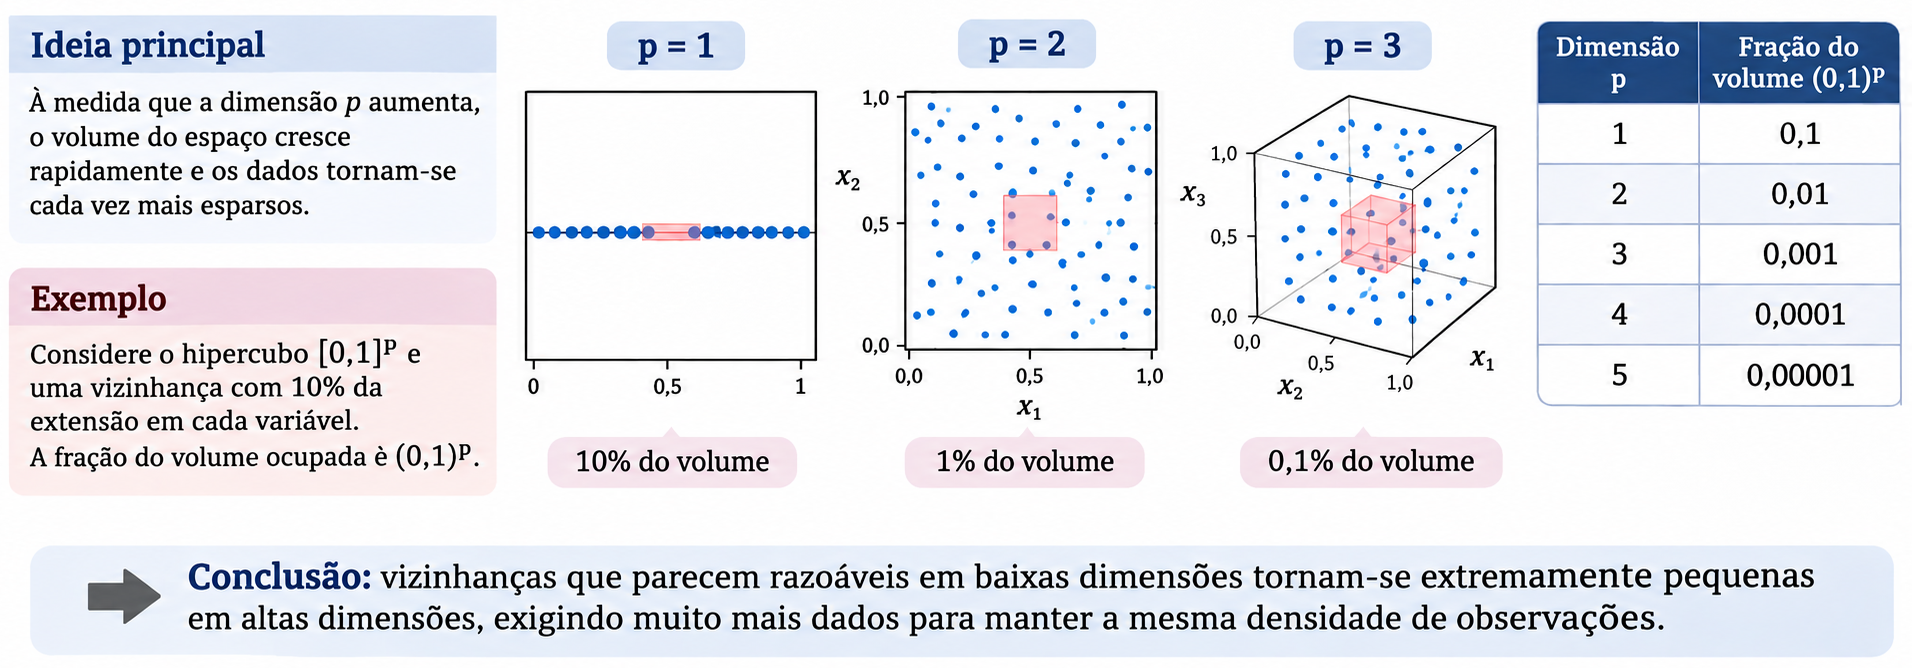
\includegraphics[width=1\linewidth,height=\textheight,keepaspectratio]{../../images/regressao/dim_e frac_de_volume.png}
\end{frame}

\begin{frame}{A maldição da dimensionalidade}
\phantomsection\label{a-maldiuxe7uxe3o-da-dimensionalidade-1}
Para manter \(k\) observações \textbf{em média} nessa região:

\[
\boxed{nh^p=k\quad\Longrightarrow\quad n=\frac{k}{h^p}}
\]

Por exemplo,

\begin{longtable}[]{@{}lrrr@{}}
\toprule\noalign{}
Com \(h=0{,}1\) e \(k=20\) & \(p=1\) & \(p=3\) & \(p=5\) \\
\midrule\noalign{}
\endhead
Amostra necessária, em média & 200 & 20.000 & 2.000.000 \\
\bottomrule\noalign{}
\end{longtable}
\end{frame}

\begin{frame}{A maldição da dimensionalidade}
\phantomsection\label{a-maldiuxe7uxe3o-da-dimensionalidade-2}
Manter vizinhanças pequenas exige muito mais dados. Isso afeta
especialmente KNN e regressão local.

\textbf{Esta conta ilustra cobertura do espaço sob uniformidade. Não é
uma regra geral de tamanho amostral.}
\end{frame}

\begin{frame}{Taxa de convergência}
\phantomsection\label{taxa-de-converguxeancia}
A \textbf{taxa de convergência} descreve a velocidade com que o risco de
estimação diminui à medida que aumentamos o tamanho da amostra \(n\).

Em regressão, podemos medir esse risco pelo \textbf{erro quadrático
médio de estimação}:

\[
R_n =
\mathbb{E}\left[
\left(\hat g_n(\mathbf X)-r(\mathbf X)\right)^2
\right]
\]

em que \(\hat g_n\) é a função estimada com \(n\) observações e \(r\) é
a verdadeira função de regressão. A esperança considera a amostra de
treinamento e uma nova entrada \(\mathbf X\).
\end{frame}

\begin{frame}{Taxa de convergência}
\phantomsection\label{taxa-de-converguxeancia-1}
Uma forma comum de descrever a taxa de convergência de um estimador, é
dada por

\[
\boxed{R_n \approx Cn^{-a}, \qquad C>0,\quad a>0,}
\]

Assim, por exemplo, quadruplicar a amostra multiplica o termo principal
do erro por \(4^{-a}\).
\end{frame}

\begin{frame}{Taxa de convergência}
\phantomsection\label{taxa-de-converguxeancia-2}
\begin{longtable}[]{@{}ccc@{}}
\toprule\noalign{}
Expoente & Erro relativo & Redução do erro \\
\midrule\noalign{}
\endhead
\(a=1\) & \(0{,}25\) & \textbf{75\%} \\
\(a=1/2\) & \(0{,}50\) & \textbf{50\%} \\
\(a=1/6\) & \(0{,}79\) & \textbf{21\%} \\
\bottomrule\noalign{}
\end{longtable}

\textbf{Interpretação:} quanto menor o expoente \(a\), mais lentamente o
erro diminui com a inclusão de novas observações.
\end{frame}

\begin{frame}{Taxas de convergência e dimensionalidade}
\phantomsection\label{taxas-de-converguxeancia-e-dimensionalidade}
Para classes gerais de funções suaves em \(p\) dimensões, uma taxa
minimax típica do erro quadrático integrado é

\[
\boxed{R_n^*\asymp n^{-\frac{2\alpha}{2\alpha+p}}}
\]

\begin{itemize}
\tightlist
\item
  \(\alpha\): suavidade da função. Valores maiores impõem maior
  regularidade.
\item
  \(R_n^*\): melhor risco possível no pior caso da classe considerada.
\item
  \(\asymp\): mesma ordem, desconsiderando constantes multiplicativas.
\end{itemize}

\textbf{Aumentar \(p\) reduz o expoente e torna a aprendizagem mais
lenta.}

A taxa exige condições sobre a classe de funções, o desenho e o ruído.
Mede estimação de \(g\), sem incluir o ruído irredutível de uma nova
resposta.

\note{Formalmente, R\_n\^{}*=inf\_\{estimadores\} sup\_\{f em F\_alpha\}
E{[}(f\_estimado(X)-f(X))²{]}, com esperança sobre treinamento e nova
entrada. Taxa minimax usual sob condições de regularidade, dimensão fixa
e classe suave. Fonte: Wasserman, Nonparametric Regression.}
\end{frame}

\begin{frame}{Quanto ganhamos aumentando a amostra?}
\phantomsection\label{quanto-ganhamos-aumentando-a-amostra}
Fixando suavidade \(\alpha=2\), a taxa é \(n^{-4/(4+p)}\).

\begin{longtable}[]{@{}rrr@{}}
\toprule\noalign{}
Dimensão \(p\) & Taxa & Fator do termo principal com \(4n\) \\
\midrule\noalign{}
\endhead
1 & \(n^{-4/5}\) & \(0{,}33\) \\
4 & \(n^{-1/2}\) & \(0{,}50\) \\
10 & \(n^{-2/7}\) & \(0{,}67\) \\
20 & \(n^{-1/6}\) & \(0{,}79\) \\
\bottomrule\noalign{}
\end{longtable}

Em uma dimensão, o termo cai para cerca de 33\% do valor anterior. Em 20
dimensões, permanece em cerca de 79\%.

\textbf{Para reduzir esse termo à metade em \(p=20\), seria necessário
multiplicar \(n\) por \(2^6=64\).}
\end{frame}

\begin{frame}{A redução do erro fica mais lenta}
\phantomsection\label{a-reduuxe7uxe3o-do-erro-fica-mais-lenta}
\pandocbounded{\includegraphics[keepaspectratio]{aula_altas_dimensoes_est335_revisada_files/figure-beamer/unnamed-chunk-1-1.png}}

Todas as curvas começam em 1 para comparar \textbf{velocidades de
redução}, não níveis absolutos de erro. São curvas teóricas com
\(\alpha=2\), sem resultados de ajuste a dados.
\end{frame}

\begin{frame}{Como tornar o problema mais simples?}
\phantomsection\label{como-tornar-o-problema-mais-simples}
A taxa anterior considera uma classe ampla de funções em \(p\)
dimensões.

Podemos explorar hipóteses que reduzam a complexidade relevante:

\begin{longtable}[]{@{}
  >{\raggedright\arraybackslash}p{(\linewidth - 4\tabcolsep) * \real{0.3333}}
  >{\raggedright\arraybackslash}p{(\linewidth - 4\tabcolsep) * \real{0.3333}}
  >{\raggedright\arraybackslash}p{(\linewidth - 4\tabcolsep) * \real{0.3333}}@{}}
\toprule\noalign{}
\begin{minipage}[b]{\linewidth}\raggedright
Hipótese
\end{minipage} & \begin{minipage}[b]{\linewidth}\raggedright
Ideia
\end{minipage} & \begin{minipage}[b]{\linewidth}\raggedright
O que procuramos
\end{minipage} \\
\midrule\noalign{}
\endhead
Esparsidade & Poucas entradas são necessárias à função de predição &
Selecionar efeitos relevantes \\
Redundância & Muitas entradas carregam informação compartilhada &
Combinar ou representar informação comum \\
\bottomrule\noalign{}
\end{longtable}

\textbf{Ter muitas variáveis observadas não implica que a resposta
dependa de todas de forma independente e complexa.}
\end{frame}

\begin{frame}{Esparsidade: poucos efeitos ativos}
\phantomsection\label{esparsidade-poucos-efeitos-ativos}
Suponha \(p=1.000\), mas

\[
Y=3X_2-2X_{17}+1{,}5X_{204}+\varepsilon
\]

A função de regressão utiliza apenas \(s=3\) entradas: \(s\ll p\).

Se soubéssemos quais são, o ajuste seria muito mais simples. Como não
sabemos, precisamos encontrá-las entre as 1.000 candidatas.

\textbf{Lasso pode explorar esparsidade dos coeficientes.}
\end{frame}

\begin{frame}{Redundância: muitas medições do mesmo fenômeno}
\phantomsection\label{redunduxe2ncia-muitas-mediuxe7uxf5es-do-mesmo-fenuxf4meno}
Imagine 100 sensores que medem uma condição térmica comum:

\[
X_j=a_jZ+\eta_j,\qquad j=1,\ldots,100.
\]

\(Z\) é a condição compartilhada, \(a_j\) é a sensibilidade do sensor e
\(\eta_j\) é o ruído específico da medição.

As entradas podem ser fortemente correlacionadas. Se \(Y\) depende
principalmente de \(Z\), a informação preditiva está associada a uma
estrutura simples.

\textbf{Ridge pode estabilizar o uso conjunto dessas medições.}
\end{frame}

\section{Métodos mais adequados à alta
dimensionalidade}\label{muxe9todos-mais-adequados-uxe0-alta-dimensionalidade}

\begin{frame}{Ridge: estabilidade com muitas entradas}
\phantomsection\label{ridge-estabilidade-com-muitas-entradas}
Ridge minimiza o erro de ajuste acrescido de uma penalização quadrática:

\[
\sum_{i=1}^{n}(y_i-\beta_0-\mathbf x_i^\top\boldsymbol\beta)^2
+\lambda\sum_{j=1}^{p}\beta_j^2
\]

\textbf{Quando considerar:} entradas correlacionadas ou sinal
distribuído por muitos efeitos pequenos.

Para \(\lambda>0\), o critério produz coeficientes únicos mesmo com
\(p>n\), no ajuste com intercepto separado.

A penalização estabiliza o ajuste, mas geralmente mantém todos os
coeficientes. Uma solução única não garante boa predição: \(\lambda\)
precisa ser escolhido por validação.
\end{frame}

\begin{frame}{Lasso: regularização com seleção}
\phantomsection\label{lasso-regularizauxe7uxe3o-com-seleuxe7uxe3o}
Lasso substitui a penalização quadrática pela soma dos valores
absolutos:

\[
\sum_{i=1}^{n}(y_i-\beta_0-\mathbf x_i^\top\boldsymbol\beta)^2
+\lambda\sum_{j=1}^{p}|\beta_j|
\]

\textbf{Quando considerar:} poucos efeitos aproximadamente lineares na
representação utilizada.

O critério favorece coeficientes exatamente iguais a zero, podendo
reduzir o conjunto de entradas utilizadas.

Com entradas fortemente correlacionadas, a escolha de variáveis pode
mudar entre amostras. \textbf{Selecionar uma variável não prova que ela
seja a única portadora do sinal.}
\end{frame}

\begin{frame}{SVM linear: classificação com regularização}
\phantomsection\label{svm-linear-classificauxe7uxe3o-com-regularizauxe7uxe3o}
A SVM linear utiliza uma função de decisão

\[
g(\mathbf x)=\mathbf w^\top\mathbf x+b
\]

com controle da magnitude de \(\mathbf w\) e penalização das violações
da margem.

\textbf{Quando considerar:} classificação com muitas entradas e uma
fronteira linear plausível, inclusive em problemas com \(p>n\).

Um kernel não linear pode ampliar a flexibilidade, mas distâncias pouco
informativas não passam a ser úteis apenas pelo uso do kernel.
\end{frame}

\begin{frame}{RNA: possibilidade de aprender representações}
\phantomsection\label{rna-possibilidade-de-aprender-representauxe7uxf5es}
Uma camada oculta calcula

\[
\mathbf a^{(1)}=\phi(W^{(1)}\mathbf x+\mathbf b^{(1)}).
\]

Ela pode combinar entradas redundantes e representar relações não
lineares.

\textbf{Quando considerar:} estrutura não linear que possa ser aprendida
com os dados disponíveis, arquitetura adequada e regularização.

\begin{itemize}
\tightlist
\item
  Com \(H\) neurônios, a primeira camada já possui \(H(p+1)\)
  parâmetros.
\item
  Weight decay penaliza pesos. Early stopping controla a duração do
  ajuste pela validação.
\end{itemize}

\textbf{Uma RNA não é automaticamente uma boa escolha para \(p\gg n\).}
Com amostra pequena, ridge e lasso são referências importantes para
comparação.
\end{frame}

\begin{frame}{Qual método considerar primeiro?}
\phantomsection\label{qual-muxe9todo-considerar-primeiro}
\begin{longtable}[]{@{}
  >{\raggedright\arraybackslash}p{(\linewidth - 2\tabcolsep) * \real{0.5000}}
  >{\raggedright\arraybackslash}p{(\linewidth - 2\tabcolsep) * \real{0.5000}}@{}}
\toprule\noalign{}
\begin{minipage}[b]{\linewidth}\raggedright
Situação
\end{minipage} & \begin{minipage}[b]{\linewidth}\raggedright
Método estudado a considerar
\end{minipage} \\
\midrule\noalign{}
\endhead
Muitas entradas correlacionadas ou muitos efeitos pequenos & Ridge \\
Poucos efeitos lineares relevantes & Lasso \\
Classificação com fronteira aproximadamente linear & SVM linear
regularizada \\
Relações não lineares e dados suficientes para aprendê-las & RNA
regularizada \\
\bottomrule\noalign{}
\end{longtable}

A tabela orienta comparações, sem definir um vencedor universal.

\textbf{Procedimento essencial:} estimar padronização, seleção e
hiperparâmetros dentro do treinamento/validação. Reservar o teste para a
avaliação final.
\end{frame}




\end{document}
